\subsection{Whole Time Series Algorithms}
\label{SubsectionWhole}
Whole time series similarity algorithms, also called distance-based algorithms, are methods that compare pairs of time series instances.
An unlabeled time series instance is given the class label of the nearest instance in a training data set \cite{kate2016using}.
There are two main techniques for carrying out the comparison;
either by comparing vector representations of the time series instances,
or by combining a defined distance function with a classifier, KNN being the most common one \cite{lines2018time}.
Whole time series algorithms are best suited for problems where the unique features can exist anywhere along the whole time series\cite{bagnall2017great}.

One of the simplest forms of whole time series is 1-NN with Euclidean Distance \cite{faloutsos1994fast}, yet it can suprisingly attain high accuracy compared to other distance measures \cite{xing2010brief}.
But Nearest Neighbor with Euclidean Distance (KNNED) is an easy to beat baseline, due to it's sensitivity for distortion and inability to handle time series of unequal lengths \cite{xing2010brief,kate2016using,lines2018time}.
This lead many of the researchers to focus on defining more advanced and elastic distance measures that can compensate for misalignment between time series \cite{abanda2019review}.
The standard and most common baseline classifier utilizing elastic distance measures is 1-NN with Dynamic Time Warping (DTW) \cite{bagnall2017great}.
In contrast to the idea that more powerful machine learning algorithms will be able to defeat the simple KNN and an elastic measure,
DTW has proved to be a very tough opponent to other algorithms and other elastic distance measures as well \cite{kate2016using,lines2015time,wang2013experimental}.
But there were also other distance metrics that have been introduced in literature, these inlcude extensions of DTW on one hand like; Weighted Dynamic Time Warping (WDTW) which penalizes large warpings based on distance \cite{jeong2011weighted}
and Derivative Dynamic Time Warping (DDTW) \cite{keogh2001derivative,gorecki2013using} which uses derivatives of sequences as features rather than raw data to avoid singularities.
On the other hand, Edit Distance with Real Penalty (ERP) \cite{chen2004marriage}, Time Warp Edit (TWE) \cite{marteau2008time}, Longest Common Subsequence (LCSS) \cite{das1997finding} and Move-Split-Merge (MSM) \cite{stefan2012move}
are all alternatives for distance measures, yet multiple experiments have considered DTW to be relatively unbeatable \cite{bagnall2017great,abanda2019review,bostrom2017shapelet}.
To the extend of our knowledge, the most powerful whole time series classifiers is Proximity Forest (PF) \cite{lucas2019proximity}.

%%%%%%%%%%%%%%%%%%%%%%%%%%%%%%%%%%%%%
\subsubsection{Nearest Neighbor with ED}
The Euclidean distance is a remarkably simple technique to calculate the distance between time series instances.
Given two instances  $T_{1}$ = [$t1_{1}$,$t1_{2}$,...$t1_{n}$]
and $T_{2}$ = [$t2_{1}$,$t2_{2}$,...$t2_{n}$], the euclidean distance
between them can be determined as:
\begin{equation}
    ED(T_{1},T_{2})= \sqrt{\sum_{i=1}^{n} (t1_{i} - t2_{i})^{2}}
\end{equation}
Euclidean distnace has been preferred to other classifiers due to it's space and time efficiency, but it suffers from two main shortcomings \cite{baydogan2013bag, jeong2011weighted,kate2016using}.
The first one is that it cannot handle comparisons between time series of different lengths.
While the second one is it's sensitivity to minor discrepancies between time series; it would calculate large distance values for small shiftings or misalignments.
Although other metrics have been introduced to overcome the drawbacks of euclidean distance,
experimental proof showed that this is only the case for small datasets, but for larger datasets the accuracy of other elastic measures
converge with euclidean distance \cite{hills2014classification,ding2008querying,bagnall2012transformation}.


%%%%%%%%%%%%%%%%%%%%%%%%%%%%%%%%%%%%%
\subsubsection{Nearest Neighbor with DTW}
\label{SubsubsectionDTW}
Dynamic Time Warping was a very strong baseline for time series classification for a long time \cite{abanda2019review,bagnall2017great}.
It was first introduced as a technique to recognize spoken words that can deal with misallignments between time series
that Euclidean Distance couldn't handle \cite{tan2020fastee}.
Figure \ref{Img:ED_vs_DTW} shows a comparison between ED and DTW while computing the distance between two time series instances.

\begin{figure}[!htbp]
    \captionsetup{justification=raggedright}
    \centering
    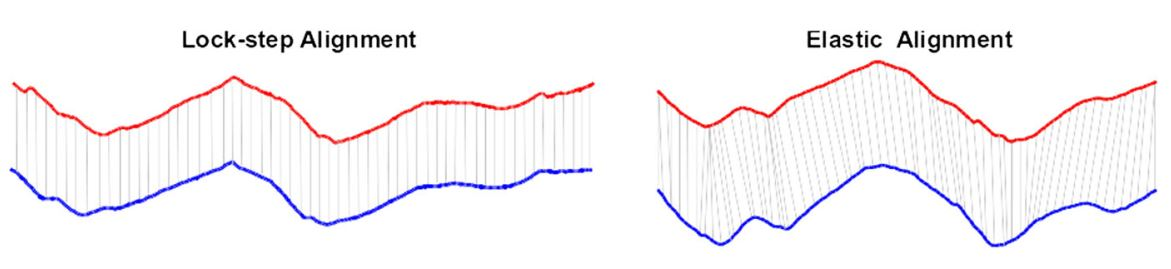
\includegraphics[scale = 0.5]{ED_vs_DTW.JPG}
    \centering
    \caption{Mapping of Euclidean distance (lock-step measure) versus mapping of DTW distance (elastic measure) \cite{abanda2019review}.}
    \label{Img:ED_vs_DTW}
\end{figure}

To calculate the distance between two time series instances  $T_{1} = [t1_{1},t1_{2},...t1_{n}$]
and $T_{2} = [t2_{1},t2_{2},...t2_{n}$];
a distance matrix $M(T_{1},T_{2})$, of size n $\times$ n, is calculated for $T_{1}$ and $T_{2}$.
With $M_{i,j}(t1_{i},t2_{j})$ representing the distance between $t1_{i}$ $\in$ $T_{1}$
and $t2_{j}$ $\in$ $T_{2}$.
The goal of DTW is to find an optimal path that minimizes the cumulative distance between points of $T_{1}$ and $T_{2}$.

A candidate path $P = [p_{1},p_{2},...p_{p}]$ is to be found by traversing M.
For a path to be valid it must conform to three conditions:
\begin{itemize}
    \item $p_{1} = (t1_{1},t2_{1})$
    \item $p_{p} = (t1_{n},t2_{n})$
    \item for all i \textless m :
        \begin{itemize}
            \item $0 \leq t1_{i+1} - t1_{i} \leq 1$
            \item $0 \leq t2_{i+1} - t2_{i} \leq 1$
        \end{itemize}
\end{itemize}

Finding an optimal path under DTW can be computationally expensive with complexity of $O(n^2)$ for a time series of length n \cite{schafer2017fast,petitjean2016faster}.
Consequently it is usual to use a contraint with the path; to prevent comparison of points outside a certain window \cite{tan2020fastee}; like the famous Sakoe-Chiba Band \cite{sakoe1978dynamic}, Itakura Parallelogram \cite{itakura1975minimum} and Ratanamahatana-Keogh Band \cite{ratanamahatana2004making}.
Typically DTW can make use of it's warping window to handle distortion in time series,
but still it is vulnerable to cases where the difference in length between instances length is larger than the warping window \cite{tan2019time}.

%%%%%%%%%%%%%%%%%%%%%%%%%%%%%%%%%%%%%
\subsubsection{Nearest Neighbor with MSM Distance}
\label{SubsubsectionMSM}
Move-Split-Merge is distance measure that was first introduced in \cite{stefan2012move}.
The main purpose of introducing MSM was to combine certain characteristics within one distance measure.
These are; robustness to misalignments between time series instances, being an actual metric unlike other distance measures like DTW and LCSS,
assure translation invariance and achieve quadratic run-time \cite{lines2015time}.

The way MSM works is pretty much like other edit distance methods; it determines the similarity between two instances
through the usage of a set of operations to transform one of them to the other. These operations, as the name indicates, are; move, split and merge \cite{bagnall2017great}.

Move is the substitution of one single time point of a series with another.
Split divides a single time point of a series into two consecutive time points holding the same value as the originial time point.
Merge can be seen as the opposite of Split, it combines two consecutive time points holding the same value into one time point.

\begin{figure}[!htbp]
    \captionsetup{justification=raggedright}
    \centering
    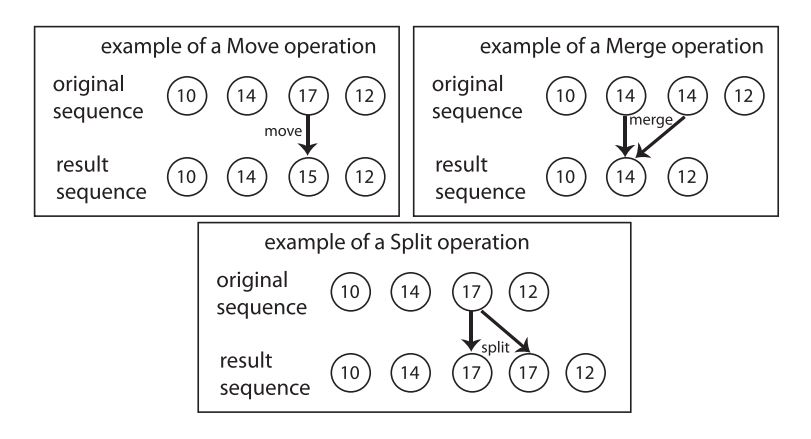
\includegraphics[scale = 0.5]{MSM.JPG}
    \centering
    \caption{Examples of the Move, Split, Merge operations \cite{stefan2012move}.}
    \label{Img:MSM}
\end{figure}

Each of the previously mentioned operations is associated with a cost.
The cost of a move is equal to the absolute difference between the old and the new value of the time point.
The costs of split and merge are equal and they are set to a constant to satisfy the symmetry property of metricity \cite{stefan2012move,tan2020fastee}.
%%%%%%%%%%%%%%%%%%%%%%%%%%%%%%%%%%%%%
\subsubsection{Proximity Forest}
\label{SubsubsectionPForest}
Proximity forest was developed by \cite{lucas2019proximity}.
It was introduced as an addition to scalable time series classification, offering a more scalable and accurate classifier than EE \cite{tan2020fastee}.
On one side, EE was an accurate classifier being one the state of the art algorithms and the best among distnace based algorithms, as it combines 11 NN-algorithms each using a different elastic measure.
But on the other hand, EE's training process was very slow as it scales quadratically with the training size of the data set \cite{lines2015time,bagnall2017great}.
This goes back to the leave-one-out-cross-validation (LOOCV) used to optimize the parameters for each used metric \cite{shifaz2020ts}.

Proximity Forest wanted to achieve two main goals. The first was to offer an adaptable algorithm that can scale with huge data sets consisting of millions of time series instances.
Beating EE, by orders of maginute, and other state of the art algorithms in terms of training and testing run time complexity.
While the other goal was to develop a competitive algorithm on the UCR data sets archive without the need to sacrifice accuracy for scalability as is the case with BOSS-VS \cite{lucas2019proximity}.


Capitalizing on the previous research that has been put in developing specialized time series distance measures and inspired by the existing EE \cite{fawaz2020inceptiontime,fawaz2019deep}.
Proximity forests combine the the eleven elastic distances from EE along with a tree-based algorithms to form an ensemble of decision trees.
The reason behind using tree-based algorithms lies in the divide-and-conquer strategy that they adopt, which makes them scalable for large data sets.
Also a stochastic process is used for the selection of distance measures and their hyper-parameters, which usually hinders the performance of other algorithms,
like KNN, that need to learn the hyper-parameters of the utilized distance measure for each data set before using it \cite{lucas2019proximity}.
Proximity forests can scale sublinearly with training data set size, but quadratically with the length of the time series \cite{shifaz2020ts}.

%\subsection{Learning a proximity forest}
Proximity forests are based on a similar concept as Random Forests \cite{breiman2001random}, another tree-based ensemble, which learns only on a subset of the available features
for building tree nodes. This process insinuates in a factor of variability between the trees that form the ensemble but each with a low bias.
The collective classification accuracy of the ensemble then tends to provide better results than any if it's single classifiers \cite{lucas2019proximity}.

The building unit of a proximity forest is called the proximity tree. A proximity tree and a decision tree are similar on all aspects,
but they differ in the tests they apply in internal nodes.
A conventional decision tree builds it's nodes using attributes. When an instance is being tested, it is compared to the value of the attribute
and then follows the branch to which it conforms.

Unlike conventional decision trees, that use feature values for their nodes, proximity trees build their nodes using randomly selected examplars.
When an instance to be tested, an elastic distance measure is calculated and then it follows the branch of the nearest examplar.

An internal node in the tree holds two attributes; \emph{measure} and \emph{branches}.
As noted in \cite{lucas2019proximity}, a measure is function \emph{object} $\times$ \emph{object} $\rightarrow\mathbb{R}$.
Proximity Forest uses the same 11 distance measures used by EE; Euclidean distance (ED) Dynamic time warping using the full window (DTW);
Dynamic time warping with a restricted warping window (DTW-R); Weighted dynamic time warping (WDTW);
Derivative dynamic time warping using the full window (DDTW); Derivative dynamic time warping with a restricted warping window (DDTW-R);
Weighted derivative dynamic time warping (WDDTW); Longest common subsequence (LCSS); Edit distance with real penalty (ERP);
Time warp edit distance (TWE); and, Move-Split-Merge (MSM).
Proximity Forest saves a lot of the computational cost by replacing parameter searches with random sampling \cite{fawaz2020inceptiontime,fawaz2019deepreview}.
While branches is a vector of the possible branches to follow, each branch holding two attributes; \emph{examplar} and \emph{subtree}.
\emph{examplar} is a time series instance to which a query instance is compared, and \emph{subtree} refers to the tree an instance should follow
in case it is closest to a specific examplar.

If all time series in a specific node share the same class, then a leaf node is created and the value of the class label is assigned to the \emph{class}
attribute of this node. During classification, if a query instance is to reach this node, it is directly labeled with the value of it's \emph{class} attribute.

%\subsection{Classifying with a proximity forest}
When a query time series is to be classified, it starts at the root node of a proximity tree.
The distance between the query and each of the randomly selected examplars is calculated, using the randomly selected distance measure at the node.
Then the query travels down the branch of the nearest examplar. This processes is repeated, passing through the internal nodes of the tree
till the query reaches a leaf node, where it is assigned the class label of that node. This whole process is then repeated for all the trees
constituting the forest. The final classification of the forest is made by majority voting between it's trees.

\begin{figure}[!htbp]
    \captionsetup{justification=raggedright}
    \centering
    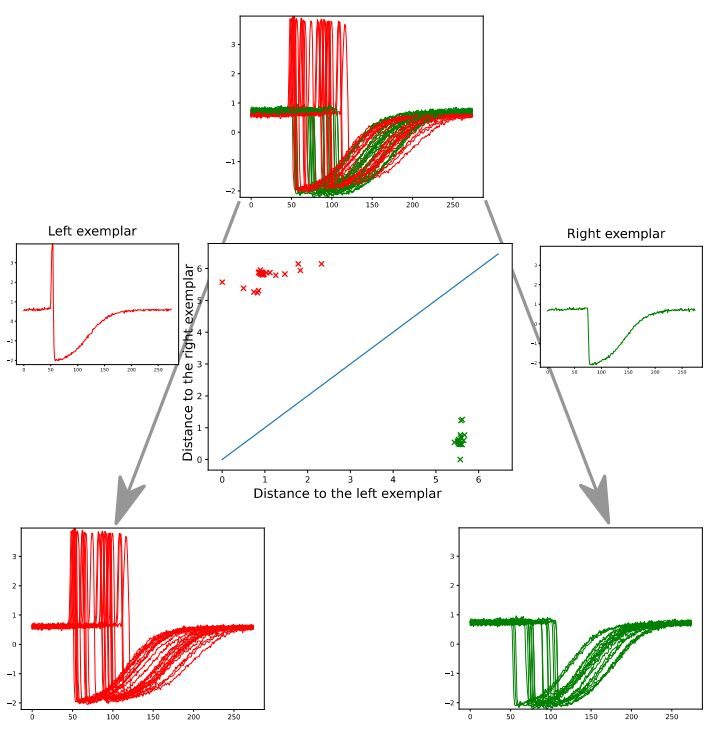
\includegraphics[scale = 0.5]{PForest.JPG}
    \caption{Visual depiction of the root node for the ‘Trace’ dataset (simplified to 2 classes). The top chart represents the data at the root node (one colour per class) while the data at the bottom left and right represent the data once split by the tree. The two time series in the middle left and right are the exemplars on which the tree is splitting. The scatter plot at the center represents the distance of each time series at the root node with respect to the left and right exemplars (resp. x- and y-axes) (Color figure online) \cite{lucas2019proximity}.}
    \label{Img:PForest}
\end{figure}


